\documentclass[10pt]{article}


\usepackage{times}
\usepackage{amsfonts}
\usepackage{amsmath}
\usepackage[psamsfonts]{amssymb}
\usepackage{latexsym}
\usepackage{color}
\usepackage{graphics}
\usepackage{enumerate}
\usepackage{amstext}
\usepackage{blkarray}
\usepackage{url}
\usepackage{epsfig}
\usepackage{bm}
\usepackage{hyperref}
\hypersetup{
    colorlinks=true,
    linkcolor=blue,
    filecolor=magenta,      
    urlcolor=blue,
}
\usepackage{mathtools}
 
\def\Kset{\mathbb{K}}
\def\Nset{\mathbb{N}}
\def\Qset{\mathbb{Q}}
\def\Rset{\mathbb{R}}
\def\Sset{\mathbb{S}}
\def\Zset{\mathbb{Z}}
\def\squareforqed{\hbox{\rlap{$\sqcap$}$\sqcup$}}
\def\qed{\ifmmode\squareforqed\else{\unskip\nobreak\hfil
\penalty50\hskip1em\null\nobreak\hfil\squareforqed
\parfillskip=0pt\finalhyphendemerits=0\endgraf}\fi}

\DeclareMathOperator*{\E}{\rm E}
\DeclareMathOperator*{\argmax}{\rm argmax}
\DeclareMathOperator*{\argmin}{\rm argmin}
\DeclareMathOperator{\sgn}{sign}
\DeclareMathOperator{\supp}{supp}
\DeclareMathOperator{\last}{last}
\DeclareMathOperator{\sign}{\sgn}
\DeclareMathOperator{\diag}{diag}
\providecommand{\abs}[1]{\lvert#1\rvert}
\providecommand{\norm}[1]{\lVert#1\rVert}
\def\vcdim{\textnormal{VCdim}}
\DeclareMathOperator*{\B}{\textbf{B}}

\DeclarePairedDelimiter\ceil{\lceil}{\rceil}
\DeclarePairedDelimiter\floor{\lfloor}{\rfloor}

\newcommand{\cX}{{\mathcal X}}
\newcommand{\cY}{{\mathcal Y}}
\newcommand{\cA}{{\mathcal A}}
\newcommand{\ignore}[1]{}
\newcommand{\bi}{\begin{itemize}}
\newcommand{\ei}{\end{itemize}}
\newcommand{\be}{\begin{enumerate}}
\newcommand{\ee}{\end{enumerate}}
\newcommand{\bd}{\begin{description}}
\newcommand{\ed}{\end{description}}
\newcommand{\h}{\widehat}
\newcommand{\e}{\epsilon}
\newcommand{\mat}[1]{{\mathbf #1}}
\newcommand{\R}{\mat{R}}
\newcommand{\0}{\mat{0}}
\newcommand{\M}{\mat{M}}

\newcommand{\D}{\mat{D}}
\renewcommand{\r}{\mat{r}}
\newcommand{\x}{\mat{x}}
\renewcommand{\u}{\mat{u}}
\renewcommand{\v}{\mat{v}}
\newcommand{\w}{\mat{w}}
\renewcommand{\H}{\text{0}}
\newcommand{\T}{\text{1}}
\newcommand{\set}[1]{\{#1\}}
\newcommand{\xxi}{{\boldsymbol \xi}}
\newcommand{\ssigma}{{\boldsymbol \sigma}}
\newcommand{\Alpha}{{\boldsymbol \alpha}}
\newcommand{\tts}{\tt \small}
\newcommand{\hint}{\emph{hint}}
\newcommand{\matr}[1]{\bm{#1}}     % ISO complying version
\newcommand{\vect}[1]{\bm{#1}} % vectors

\newcommand{\Var}{\mathrm{Var}}
\newcommand{\Cov}{\mathrm{Cov}}

% New commands
\newcommand{\SP}{\mathbf{S}_{+}^n}
\newcommand{\Proj}{\mathcal{P}_{\mathcal{S}}}
\DeclarePairedDelimiterX{\inp}[2]{\langle}{\rangle}{#1, #2}


\newenvironment{solution}{\vspace{.25cm}\noindent{\it Solution:}}{}

\begin{document}

\noindent DS-GA.1013 Mathematical Tools for Data Science :\\
Homework Assignment 0 \\
Yves Greatti - yg390\\

\begin{enumerate}
\item Projections

\be
	\item False
	Consider 
	$\vect{b_1} = \begin{bmatrix} 0\\ 1\end{bmatrix}$ and $\vect{b_2} = \begin{bmatrix} 1\\ 2\end{bmatrix}$, they form a basis of $\mat{R}^2$.
	When using the definition $\Proj x = \sum_{i=1}^n \langle x, b_i \rangle b_i$ we would expect that $\Proj b_1 = b_1$. However $\Proj b_1 = \begin{bmatrix} 2\\ 5\end{bmatrix} \neq b_1$.
	\item True
	Let $S^\bot = \{x |  \langle x,y  \rangle  = 0, \forall y \in S \}$ a subspace of an inner product space $X$, then $S^{\bot\bot} = \{x |  \langle x,y  \rangle  = 0, \forall y \in S^\bot \}$. The inner product being symmetric, $S \subseteq S^{\bot\bot}$.
	Since for any vector $x \in X$, we have $x = y + z$ where $y \in S, z \in S^\bot$, using Gram-schmidt orthonormalization process, we can find a basis of $S$ and $S^\bot$ which express any vector of X as a linear combination
	of these two basis and combining these two basis together forms a new basis for X so $\dim X = \dim S + \dim S^\bot$. If $\dim X = n$ and $\dim S = m$ then $\dim S^\bot = n - m$.
	Similarly $\dim S^{\bot\bot} = n  - (n- m) = m$ so $\dim S^{\bot\bot} = \dim S$, so $S^{\bot\bot} \subseteq S$  and since the dimension of a space or subspace is the cardinality of its basis, thus $S = S^{\bot\bot}$.
	\item True consider $\vect{v} = \begin{bmatrix} v_1\\ \vdots\\ v_n\end{bmatrix}$, we want $\vect{w} = \begin{bmatrix} \frac{\sum_{i=1,n} v_i}{n}\\ \vdots\\ \frac{\sum_{i=1,n} v_i}{n}\end{bmatrix}$. The orthogonal projection
	of $\vect{v}$ onto the vector $\vect{b}$ is defined as $\frac{v . b} {\| b \|^2}$, take  $b= \begin{bmatrix} 1\\  \vdots\\1 \end{bmatrix}$.
\ee

\item Eigen decomposition
Rewriting the problem in a matrix form: 
$$
\begin{pmatrix}
	d_{n+1} \\
	w_{n+1}
\end{pmatrix}
= \frac{1}{4}
\begin{pmatrix}
	5 & -3 \\
	1 & 	1
\end{pmatrix}
\begin{pmatrix}
	d_n \\
	w_n
\end{pmatrix}
$$
Let  $A = \frac{1}{4}
\begin{pmatrix}
	5 & -3 \\
	1 & 	1
\end{pmatrix}$, $v_{n+1} = \begin{pmatrix}
	d_{n+1} \\
	w_{n+1}
\end{pmatrix}$, $v_0 =  \begin{pmatrix} d_0 \\ w_0 \end{pmatrix}$ then $v_{n+1}= A v_n = A^n v_0$. We are looking to find the eigen decomposition so we can understand the behavior of $v_n$ as $n \rightarrow \infty$.
$\det(A - \lambda I) =  \frac{1}{2}  (2 \lambda^2 -3 \lambda + 1)$, we find for eigenvalues $\lambda_1=\frac{1}{2}$ and $\lambda_2=1$ with corresponding eigenvectors 

$w_1=\begin{pmatrix} 1 \\ 1 \end{pmatrix}, w_2 = \begin{pmatrix} 3 \\ 1 \end{pmatrix}$. Since A is diagonalizable the vectors $\{w_1, w_2\}$ forms a basis of $\mathbf{R}^2$ 
and we can express $v_0$ in this basis as $v_0 = \alpha w_1 + \beta w_2$ for some $\alpha,\beta \in \mathbf{R}$, 
thus $v_{n+1} = \alpha A^n w_1 + \beta A^n w_2 = \alpha \lambda_1^n w_1 + \beta \lambda_2^n w_2 = \alpha (\frac{1}{2^n}) w_1 + \beta w_2$. Then taking the $n\to\infty$, the first term goes to zero and $v_{n+1} \sim \beta w_2$. So asymptotically $\frac{d_{n+1}} {w_{n+1}} \sim 3$ which verifies the initial condition: $w_0 < d_0$. 
 
\item Function approximation

\be
	\item Using Gram-Schmidt orthonormalization process, we find
	\begin{align*}
		v_1 	&=	1 \\
		v_2	&= 	x - \inp{x}{1} \frac{1}{\inp{1}{1}} \\
			&= 	x \\
		v_3 	&= 	x^2 -  \inp{x^2}{v_2} \frac{v_2} {\inp{v_2} {v_2}} - \inp{x^2}{v_1} \frac{v_1}{\inp{v_1} {v_1}} \\
			&= x^2 - \frac{1}{3}
	\end{align*}
	Then we normalize each of these vectors to obtain:
	\begin{align*}
		w_1 &=	\frac{v_1}{\|v_1\|}	= \frac{\sqrt{2}}{2} \\
		w_2	&=	\frac{v_2}{\|v_2\|}	= \sqrt{\frac{3}{2}} \; x \\
		w_3	&=	\frac{v_3}{\|v_3\|}	= \sqrt{\frac{45}{8}} \; (x^2 - \frac{1}{3})
	\end{align*}

	\item The projection of $f(x) = \cos(\frac{\pi}{2} \; x )$ in the orthonormal basis $\{w_1, w_2, w_3 \}$ is: $\sum_{i=1,3} \inp{f}{w_i} w_i$, where:
	\begin{align*}
		\inp{f}{w_1}	&=	\int_{-1}^1	\cos(\frac{\pi}{2} \; x)  \; \frac{\sqrt{2}}{2} \; dx \\
					&= 	\frac{4}{\pi \sqrt{2}}	\sim 0.9 \\
		\inp{f}{w_2}	&=	\int_{-1}^1	\cos(\frac{\pi}{2} \; x)  \; \frac{\sqrt{3}}{2} \; x \; dx \\
					&= 	0 \\
		\inp{f}{w_3}	&=	\int_{-1}^1	\cos(\frac{\pi}{2} \; x) \sqrt{\frac{45}{8}} \; (x^2 - \frac{1}{3}) \; dx \\
					&= 	2 \sqrt{10} \frac{\pi^2 -12}{\pi^3}		\sim -0.43 \\					
	\end{align*}	
	
	\item
	\begin{center}
		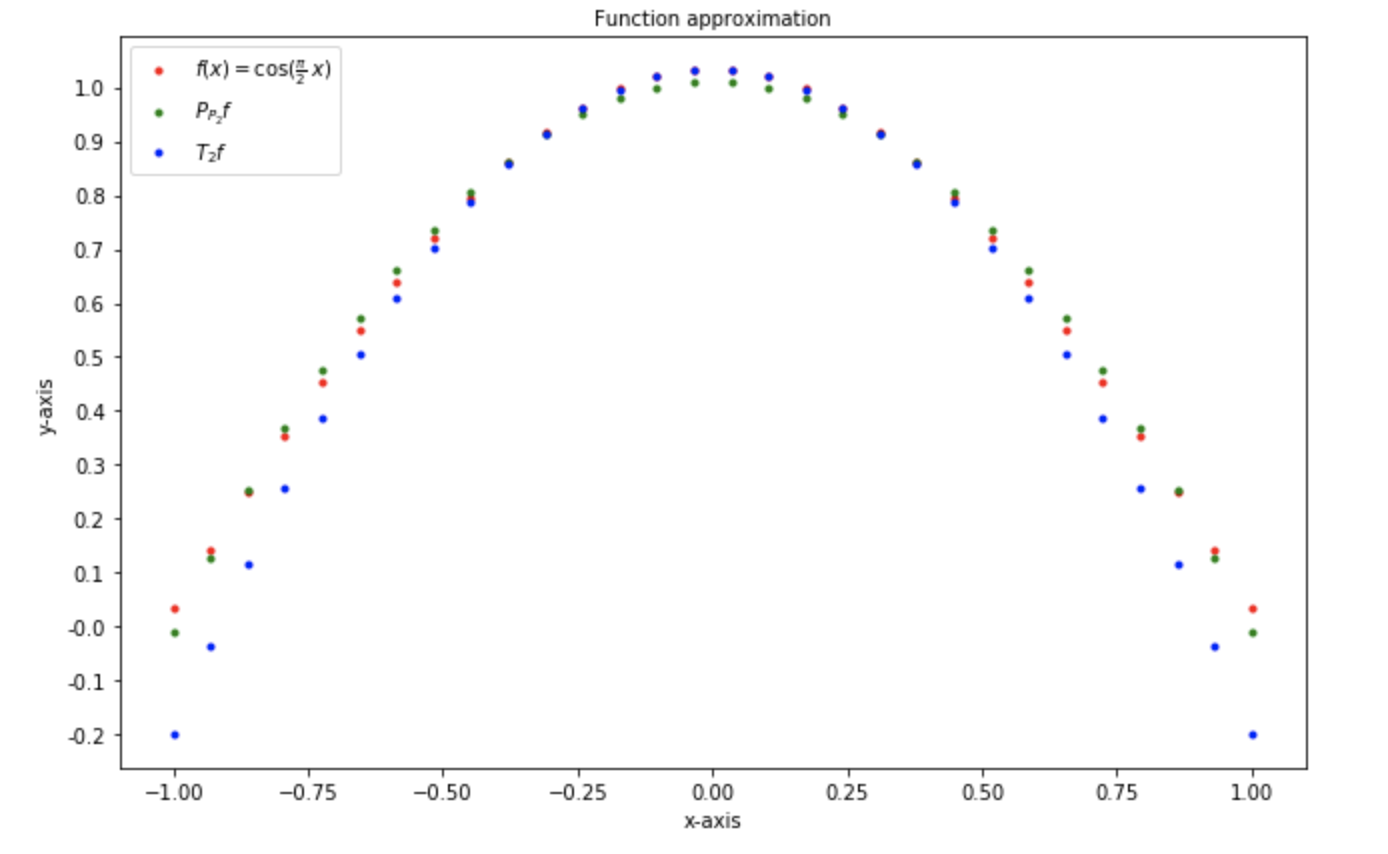
\includegraphics[width=1\linewidth]{figures/problem_3_1.png} 
	\end{center}
	
	\item $\mathcal{P}_{P2} f$is the orthogonal projection of $f(x)$ over the subspace of polynomials of degree 2: $\{ w_1, w_2, w_3 \}$, like the Taylor expansion $\mathcal{T}_2 f$, The difference is that the Taylor is a polynomial expansion of $f$ at 0. So in a neighborhood of $0$, there is almost no differences between $f$ and $\mathcal{T}_2 f$, but as we move away the approximation given  by $\mathcal{T}_2 f$ is worst than  $\mathcal{P}_{P2} f$. 
\ee	

\item Scalar linear approximation
\be
	\item First we write $\E[(a x + b - y)^2] = \E[((a x -y) - (-b))^2]$, we know that the best mean-squared error mimimizer of a random variable is its mean so $-b=\E[ax-y] = a \E[x] - \E[y]= a \mu_x - \mu_y$.
	Substituting b in the expression we want to minimize gives us:
	\begin{align*}
		\E[(a x + b - y)^2] 	&= \E[ ( a x - y -  ( a \mu_x - \mu_y) )^2 ] \\
						&= \E[ \{ a (\mu_x - x)  - (y-\mu_y)  \}^2 ] \\
						&= a^2 \E[(x - \mu_x)^2]  + \E[ (y-\mu_y)^2]  -2 a \E[(x - \mu_x) (y-\mu_y)] \\
						&= a^2 \sigma_x^2 + \sigma_y^2 -2\, a\, \Cov(x,y)
	\end{align*}
	Let $f(a) =  a^2 \sigma_x^2 + \sigma_y^2 -2\, a\, \Cov(x,y)$, then $f'(a) = 2 (\sigma_x^2 a - \Cov(x,y))$ and $f''(a) = 2 \sigma_x^2 $.
	The function is strictly convex, and its second derivative is positive, thus its minimizer is $a = \frac{ \Cov(x,y)} {\sigma_x^2} = \rho_{x,y}\, \frac{\sigma_y}{\sigma_x}$.
	
	\item Applying the result from the previous question, the best linear estimate of y given x is $y = \rho_{x,y}\, \frac{\sigma_y}{\sigma_x} (x - \mu_x)  + \mu_y$.
	Notice that $\Var{(x)} = \Var{(y \; z)} = \E{[y^2 \; z^2]} - \E{[y \; z]}^2 = \E{[y^2]}  \E{[z^2]} - \E{[y]}^2  E{[z]}^2 = (\sigma_y^2 + \mu_y^2) \sigma_z^2$ where we have used that a and z are independent and z has zero-mean. And $\E{[x]} = \E[y \; z] = \E[y] \; . \; 0 = 0$. Thus the  best linear estimate of y given x is: $\rho_{x,y} \frac{\sigma_y} {\sigma_z \sqrt{\sigma_y^2 + \mu_y^2}} \; x + \mu_y$.
	 
	 \item If in the expression above of y given x, z is normally distributed with $\sigma_z =1$ then y is estimated perfectly from x.  
	 %The mean squares error of the linear estimation above is: 
	 %$\E[(a x + b - y)^2] =  a^2 \sigma_x^2 + \sigma_y^2 -2\, a\, \Cov(x,y) =  \sigma_y^2  + a^2 \sigma_x^2 -2 a^2  \sigma_x^2 =  \sigma_y^2 -a^2 \sigma_x^2  = (1 - \rho_{y z,y})   \sigma_y^2$.
	 
\ee

\item Gradients
\be
	\item Compute the gradient of $f(x) = b^T x$ where $b \in \mathbf{R}^d$ and $f: \mathbf{R}^d \rightarrow \mathbf{R}$.
	$\frac{\partial f(x)}{x_j} = \sum_i b_i \frac{\partial x_i} {\partial x_j} = b_i$, thus $\nabla f(x) = b$.
	\item Compute the gradient of $f(x) = x^T A x$ where $A \in  \mathbf{R}^{d \times s}$ and $f: \mathbf{R}^d \rightarrow \mathbf{R}$.
	$f(x)	=  x^T A x = \sum_{i=1}^d \sum_{j=1}^d a_{ij} x_i x_j$, then
	\begin{align*}
		\frac{\partial f} {\partial x_k}	&=	\sum_{i=1}^d \sum_{j=1}^d a_{ij} \frac {\partial x_i x_j} {x_k}\\
								&=	\sum_{i=1}^d \sum_{j=1}^d a_{ij} (x_j \delta_{ik} + x_i \delta_{jk}) \\
								&=	\sum_{i=1}^d \sum_{j=1}^d a_{ij} x_j \delta_{ik}  + \sum_{i=1}^d \sum_{j=1}^d a_{ij} x_i \delta_{jk} \\
								&=	\sum_{j=1}^d  a_{kj} x_j +  \sum_{i=1}^d a_{ik}  x_i \\
								&=	(A x)_k + (A x)_k^T
	\end{align*}
	thus $\nabla f(x) = (A + A^T) x$.
\ee

\end{enumerate}

\end{document}
